%==========================================================
% CHAPTER 1: Trigonometrija
%==========================================================
\chapter{Trigonometrija}

\section{Trigonometrinių funkcijų savybės ir grafikai}

\subsection{Trigonometrinės funkcijos vienetiniame apskritime}

\begin{definition}
Vienetinis apskritimas – tai apskritimas, kurio centras koordinačių pradžioje \(O(0,0)\) ir spindulys \(r = 1\). Kiekvienam kampui \(\alpha\) (matuojamam radianais ar laipsniais) atitinka taškas \(P(\cos\alpha,\, \sin\alpha)\) ant vienetinio apskritimo.
\end{definition}

Kampas \(\alpha\) matuojamas nuo teigiamos \(Ox\) ašies prieš laikrodžio rodyklę. Radianų ir laipsnių ryšys:
\[
\alpha_{\text{rad}} = \frac{\pi}{180^\circ} \cdot \alpha_{\text{laipsniai}}, \qquad \alpha_{\text{laipsniai}} = \frac{180^\circ}{\pi} \cdot \alpha_{\text{rad}}.
\]

\begin{tcolorbox}[title=Pagrindiniai kampų radianai]
\[
0,\quad \frac{\pi}{6},\quad \frac{\pi}{4},\quad \frac{\pi}{3},\quad \frac{\pi}{2},\quad \pi,\quad \frac{3\pi}{2},\quad 2\pi
\]
atitinka laipsnius:
\[
0^\circ,\quad 30^\circ,\quad 45^\circ,\quad 60^\circ,\quad 90^\circ,\quad 180^\circ,\quad 270^\circ,\quad 360^\circ.
\]
\end{tcolorbox}

\subsection{Trigonometrinių funkcijų apibrėžimai}

\begin{definition}
Taškas \(P\) vienetiniame apskritime atitinka kampą \(\alpha\). Apibrėžiame:
\begin{align*}
\sin\alpha &= y\text{-koordinatė taško }P,\\
\cos\alpha &= x\text{-koordinatė taško }P,\\
\tan\alpha &= \frac{\sin\alpha}{\cos\alpha}, \quad \cos\alpha \neq 0,\\
\cot\alpha &= \frac{\cos\alpha}{\sin\alpha}, \quad \sin\alpha \neq 0.
\end{align*}
\end{definition}

\begin{tcolorbox}[title=Ypatingų kampų reikšmių lentelė]
\[
\begin{array}{c|c|c|c|c|c}
\alpha & 0 & \dfrac{\pi}{6} & \dfrac{\pi}{4} & \dfrac{\pi}{3} & \dfrac{\pi}{2} \\[8pt]
\hline
\sin\alpha & 0 & \dfrac{1}{2} & \dfrac{\sqrt{2}}{2} & \dfrac{\sqrt{3}}{2} & 1 \\[8pt]
\hline
\cos\alpha & 1 & \dfrac{\sqrt{3}}{2} & \dfrac{\sqrt{2}}{2} & \dfrac{1}{2} & 0 \\[8pt]
\hline
\tan\alpha & 0 & \dfrac{1}{\sqrt{3}} & 1 & \sqrt{3} & \text{n.a.} \\[8pt]
\hline
\cot\alpha & \text{n.a.} & \sqrt{3} & 1 & \dfrac{1}{\sqrt{3}} & 0 \\[8pt]
\end{array}
\]
\end{tcolorbox}

\subsection{Pagrindinės trigonometrinės tapatybės}

Iš vienetinio apskritimo apibrėžimo tiesiogiai išplaukia fundamentali tapatybė:
\[
\sin^2\alpha + \cos^2\alpha = 1.
\]

Iš jos gauname papildomas tapatybes:
\begin{align}
1 + \tan^2\alpha &= \frac{1}{\cos^2\alpha}, \quad \cos\alpha \neq 0, \\[4pt]
1 + \cot^2\alpha &= \frac{1}{\sin^2\alpha}, \quad \sin\alpha \neq 0.
\end{align}

\begin{tcolorbox}[title=Sumos ir skirtumo formulės]
\begin{align*}
\sin(\alpha \pm \beta) &= \sin\alpha\cos\beta \pm \cos\alpha\sin\beta,\\
\cos(\alpha \pm \beta) &= \cos\alpha\cos\beta \mp \sin\alpha\sin\beta,\\
\tan(\alpha \pm \beta) &= \frac{\tan\alpha \pm \tan\beta}{1 \mp \tan\alpha\tan\beta}.
\end{align*}
\end{tcolorbox}

\begin{tcolorbox}[title=Dvigubo kampo formulės]
\begin{align*}
\sin 2\alpha &= 2\sin\alpha\cos\alpha,\\
\cos 2\alpha &= \cos^2\alpha - \sin^2\alpha = 1 - 2\sin^2\alpha = 2\cos^2\alpha - 1,\\
\tan 2\alpha &= \frac{2\tan\alpha}{1 - \tan^2\alpha}.
\end{align*}
\end{tcolorbox}

\subsection{Redukcijos formulės}

Redukcijos formulės leidžia bet kurio kampo trigonometrines funkcijas išreikšti per \(\alpha \in \left[0, \frac{\pi}{2}\right)\) funkcijų reikšmes.

\begin{theorem}[Redukcijos formulių taisyklė]
Išraiška \(f\!\left(\frac{\pi}{2} k \pm \alpha\right)\), kur \(k \in \mathbb{Z}\):
\begin{itemize}
    \item Jei \(k\) \textbf{lyginis}: funkcija \textbf{nesikeičia} (pvz., \(\sin \to \sin\), \(\cos \to \cos\));
    \item Jei \(k\) \textbf{nelyginis}: funkcija \textbf{keičiasi į papildomą} (\(\sin \leftrightarrow \cos\), \(\tan \leftrightarrow \cot\));
    \item Ženklas priklauso nuo pradinės funkcijos kvadranto, kuriame yra kampas.
\end{itemize}
\end{theorem}

\begin{example}
Suprastinkite \(\sin\!\left(\pi - \alpha\right)\) ir \(\cos\!\left(\frac{\pi}{2} + \alpha\right)\).
\begin{align*}
\sin(\pi - \alpha) &= \sin\alpha \quad (\text{nes } \pi - \alpha \text{ II kvadrantas, } \sin > 0),\\
\cos\!\left(\tfrac{\pi}{2} + \alpha\right) &= -\sin\alpha \quad (\text{nes } k=1 \text{ nelyginis, } \cos\to\sin,\text{ II kvadrantas}).
\end{align*}
\end{example}

\subsection{Funkcijos \texorpdfstring{\(y = \sin x\)}{y = sin x} savybės ir grafikas}

\begin{definition}
Funkcija \(f(x) = \sin x\) apibrėžta visiems realiesiems skaičiams \(x \in \mathbb{R}\).
\end{definition}

\textbf{Pagrindinės savybės:}
\begin{itemize}
    \item \textbf{Apibrėžimo sritis:} \(D = \mathbb{R} = (-\infty, +\infty)\).
    \item \textbf{Reikšmių sritis:} \(E = [-1,\, 1]\).
    \item \textbf{Periodas:} \(T = 2\pi\), t.~y. \(\sin(x + 2\pi) = \sin x\).
    \item \textbf{Lyginumas:} \textbf{nelyginė} funkcija: \(\sin(-x) = -\sin x\).
    \item \textbf{Didėjimas:} \(\left[-\frac{\pi}{2} + 2\pi k,\; \frac{\pi}{2} + 2\pi k\right]\), \(k \in \mathbb{Z}\).
    \item \textbf{Mažėjimas:} \(\left[\frac{\pi}{2} + 2\pi k,\; \frac{3\pi}{2} + 2\pi k\right]\), \(k \in \mathbb{Z}\).
    \item \textbf{Maksimumas:} \(\sin x = 1\), kai \(x = \frac{\pi}{2} + 2\pi k\).
    \item \textbf{Minimumas:} \(\sin x = -1\), kai \(x = -\frac{\pi}{2} + 2\pi k\).
    \item \textbf{Nulinės reikšmės:} \(\sin x = 0\), kai \(x = \pi k\), \(k \in \mathbb{Z}\).
    \item \textbf{Grafiko simetrija:} simetriška koordinačių pradžiai \(O(0,0)\).
\end{itemize}

\begin{figure}[h!]
\centering
% Grafikas braižomas su pgfplots:
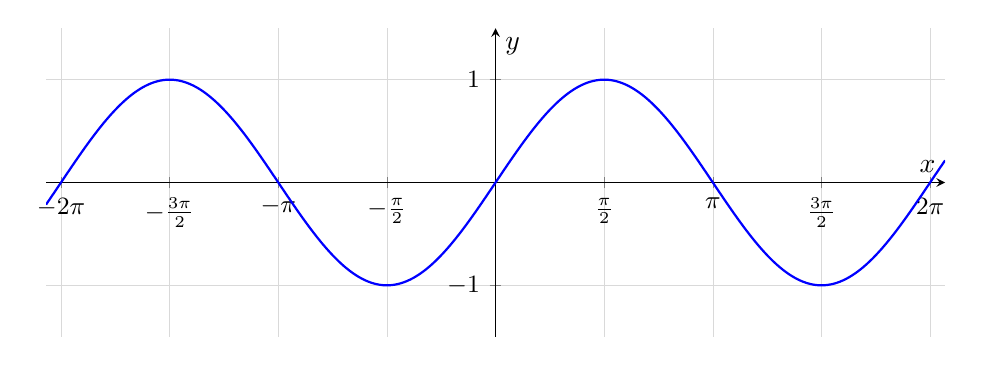
\begin{tikzpicture}
\begin{axis}[
    width=13cm, height=5.5cm,
    axis lines=center,
    xlabel={$x$}, ylabel={$y$},
    xmin=-6.5, xmax=6.5,
    ymin=-1.5, ymax=1.5,
    xtick={-6.283,-4.712,-3.14159,-1.5708,0,1.5708,3.14159,4.712,6.283},
    xticklabels={$-2\pi$,$-\frac{3\pi}{2}$,$-\pi$,$-\frac{\pi}{2}$,$0$,$\frac{\pi}{2}$,$\pi$,$\frac{3\pi}{2}$,$2\pi$},
    ytick={-1,1},
    samples=300,
    grid=both,
    grid style={line width=0.2pt, draw=gray!30},
    tick label style={font=\small},
]
\addplot[blue, thick, domain=-6.5:6.5] {sin(deg(x))};
\end{axis}
\end{tikzpicture}
\caption{Funkcijos \(y = \sin x\) grafikas}
\end{figure}

\subsection{Funkcijos \texorpdfstring{\(y = \cos x\)}{y = cos x} savybės ir grafikas}

\textbf{Pagrindinės savybės:}
\begin{itemize}
    \item \textbf{Apibrėžimo sritis:} \(D = \mathbb{R}\).
    \item \textbf{Reikšmių sritis:} \(E = [-1,\, 1]\).
    \item \textbf{Periodas:} \(T = 2\pi\), t.~y. \(\cos(x + 2\pi) = \cos x\).
    \item \textbf{Lyginumas:} \textbf{lyginė} funkcija: \(\cos(-x) = \cos x\).
    \item \textbf{Didėjimas:} \([-\pi + 2\pi k,\; 2\pi k]\), \(k \in \mathbb{Z}\).
    \item \textbf{Mažėjimas:} \([2\pi k,\; \pi + 2\pi k]\), \(k \in \mathbb{Z}\).
    \item \textbf{Maksimumas:} \(\cos x = 1\), kai \(x = 2\pi k\).
    \item \textbf{Minimumas:} \(\cos x = -1\), kai \(x = \pi + 2\pi k\).
    \item \textbf{Nulinės reikšmės:} \(\cos x = 0\), kai \(x = \frac{\pi}{2} + \pi k\), \(k \in \mathbb{Z}\).
    \item \textbf{Grafiko simetrija:} simetriška \(Oy\) ašiai.
\end{itemize}

\begin{remark}
Kosinuso grafikas yra sinuso grafiko poslinkis kairėn \(\frac{\pi}{2}\) vienetų:
\[
\cos x = \sin\!\left(x + \frac{\pi}{2}\right).
\]
\end{remark}

\begin{figure}[h!]
\centering
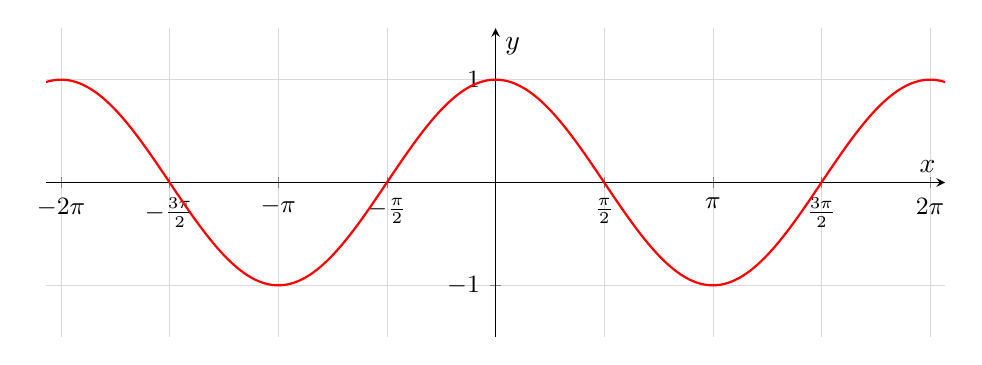
\begin{tikzpicture}
\begin{axis}[
    width=13cm, height=5.5cm,
    axis lines=center,
    xlabel={$x$}, ylabel={$y$},
    xmin=-6.5, xmax=6.5,
    ymin=-1.5, ymax=1.5,
    xtick={-6.283,-4.712,-3.14159,-1.5708,0,1.5708,3.14159,4.712,6.283},
    xticklabels={$-2\pi$,$-\frac{3\pi}{2}$,$-\pi$,$-\frac{\pi}{2}$,$0$,$\frac{\pi}{2}$,$\pi$,$\frac{3\pi}{2}$,$2\pi$},
    ytick={-1,1},
    samples=300,
    grid=both,
    grid style={line width=0.2pt, draw=gray!30},
    tick label style={font=\small},
]
\addplot[red, thick, domain=-6.5:6.5] {cos(deg(x))};
\end{axis}
\end{tikzpicture}
\caption{Funkcijos \(y = \cos x\) grafikas}
\end{figure}

\subsection{Funkcijos \texorpdfstring{\(y = \tan x\)}{y = tan x} savybės ir grafikas}

\textbf{Pagrindinės savybės:}
\begin{itemize}
    \item \textbf{Apibrėžimo sritis:} \(D = \mathbb{R} \setminus \left\{\frac{\pi}{2} + \pi k \mid k \in \mathbb{Z}\right\}\).
    \item \textbf{Reikšmių sritis:} \(E = \mathbb{R} = (-\infty, +\infty)\).
    \item \textbf{Periodas:} \(T = \pi\), t.~y. \(\tan(x + \pi) = \tan x\).
    \item \textbf{Lyginumas:} \textbf{nelyginė} funkcija: \(\tan(-x) = -\tan x\).
    \item \textbf{Didėjimas:} kiekviename intervale \(\left(-\frac{\pi}{2} + \pi k,\; \frac{\pi}{2} + \pi k\right)\).
    \item \textbf{Asimptotės:} vertikalios asimptotės \(x = \frac{\pi}{2} + \pi k\), \(k \in \mathbb{Z}\).
    \item \textbf{Nulinės reikšmės:} \(\tan x = 0\), kai \(x = \pi k\), \(k \in \mathbb{Z}\).
\end{itemize}

\begin{figure}[h!]
\centering
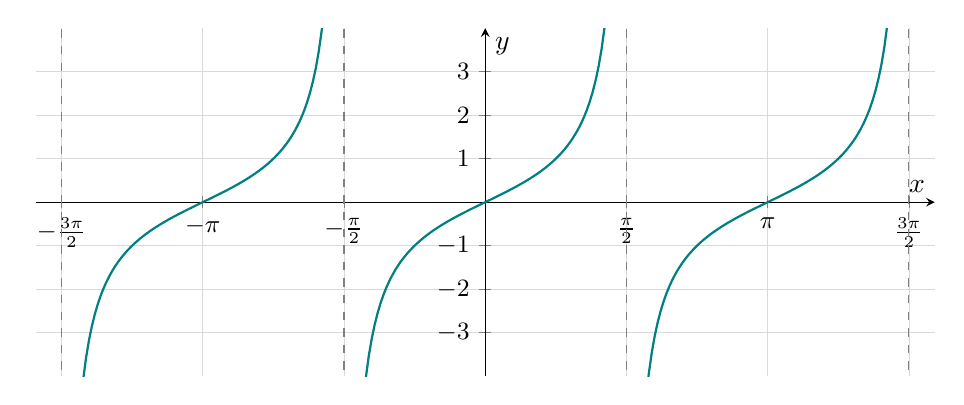
\begin{tikzpicture}
\begin{axis}[
    width=13cm, height=6cm,
    axis lines=center,
    xlabel={$x$}, ylabel={$y$},
    xmin=-5, xmax=5,
    ymin=-4, ymax=4,
    xtick={-4.712,-3.14159,-1.5708,0,1.5708,3.14159,4.712},
    xticklabels={$-\frac{3\pi}{2}$,$-\pi$,$-\frac{\pi}{2}$,$0$,$\frac{\pi}{2}$,$\pi$,$\frac{3\pi}{2}$},
    ytick={-3,-2,-1,1,2,3},
    samples=300,
    restrict y to domain=-5:5,
    grid=both,
    grid style={line width=0.2pt, draw=gray!30},
    tick label style={font=\small},
]
\addplot[teal, thick, domain=-4.9:4.9] {tan(deg(x))};
% Asimptotės
\addplot[dashed, gray, domain=-4:4] coordinates {(-1.5708,-5)(-1.5708,5)};
\addplot[dashed, gray, domain=-4:4] coordinates {(1.5708,-5)(1.5708,5)};
\addplot[dashed, gray, domain=-4:4] coordinates {(-4.712,-5)(-4.712,5)};
\addplot[dashed, gray, domain=-4:4] coordinates {(4.712,-5)(4.712,5)};
\end{axis}
\end{tikzpicture}
\caption{Funkcijos \(y = \tan x\) grafikas}
\end{figure}

\subsection{Funkcijos \texorpdfstring{\(y = \cot x\)}{y = cot x} savybės ir grafikas}

\textbf{Pagrindinės savybės:}
\begin{itemize}
    \item \textbf{Apibrėžimo sritis:} \(D = \mathbb{R} \setminus \{\pi k \mid k \in \mathbb{Z}\}\).
    \item \textbf{Reikšmių sritis:} \(E = \mathbb{R}\).
    \item \textbf{Periodas:} \(T = \pi\).
    \item \textbf{Lyginumas:} \textbf{nelyginė} funkcija: \(\cot(-x) = -\cot x\).
    \item \textbf{Mažėjimas:} kiekviename intervale \((\pi k,\; \pi + \pi k)\).
    \item \textbf{Asimptotės:} vertikalios asimptotės \(x = \pi k\), \(k \in \mathbb{Z}\).
    \item \textbf{Nulinės reikšmės:} \(\cot x = 0\), kai \(x = \frac{\pi}{2} + \pi k\), \(k \in \mathbb{Z}\).
\end{itemize}

\subsection{Keturių kvadrantų ženklai}

Priklausomai nuo to, kuriame kvadrante yra kampo galinė kraštinė, funkcijų ženklai yra:

\begin{center}
\begin{tabular}{c|c|c|c|c}
\textbf{Kvadrantas} & \textbf{I} \((0;\frac{\pi}{2})\) & \textbf{II} \((\frac{\pi}{2};\pi)\) & \textbf{III} \((\pi;\frac{3\pi}{2})\) & \textbf{IV} \((\frac{3\pi}{2};2\pi)\) \\
\hline
\(\sin\alpha\) & \(+\) & \(+\) & \(-\) & \(-\) \\
\(\cos\alpha\) & \(+\) & \(-\) & \(-\) & \(+\) \\
\(\tan\alpha\) & \(+\) & \(-\) & \(+\) & \(-\) \\
\(\cot\alpha\) & \(+\) & \(-\) & \(+\) & \(-\) \\
\end{tabular}
\end{center}

\begin{tcolorbox}[title=Mnemonika]
Pagalbinė frazė: \textbf{„Visi Studentai Tik Košę"} – ką reiškia kiekvienas žodis:
\begin{itemize}
    \item \textbf{V}isi – I kvadrante \textbf{visos} funkcijos teigiamos,
    \item \textbf{S}tudentai – II kvadrante tik \textbf{sinusas} teigiamas,
    \item \textbf{T}ik – III kvadrante tik \textbf{tangentas} (ir kotangentas) teigiami,
    \item \textbf{K}ošę – IV kvadrante tik \textbf{kosinusas} teigiamas.
\end{itemize}
\end{tcolorbox}

\subsection{Grafikų transformacijos}

Turėdami pagrindinį grafiką \(y = \sin x\), galime nagrinėti bendresnę funkciją:
\[
y = A \sin(\omega x + \varphi) + B,
\]
kur parametrų reikšmės lemia grafiko pokyčius:

\begin{itemize}
    \item \(|A|\) – \textbf{amplitudė}: grafikas ištemptas arba suspaustas vertikaliai. Reikšmių sritis tampa \([B - |A|,\; B + |A|]\).
    \item \(\omega\) – \textbf{dažnis}: periodas \(T = \dfrac{2\pi}{|\omega|}\).
    \item \(\varphi\) – \textbf{pradinė fazė}: horizontalus grafiko poslinkis \(-\dfrac{\varphi}{\omega}\) vienetų.
    \item \(B\) – \textbf{vertikalus poslinkis}: visa sinusoidė pakelta \(B\) vienetų.
    \item Jei \(A < 0\): grafikas atspindimas \(Ox\) ašies atžvilgiu.
\end{itemize}

\begin{example}
Raskite \(y = 3\sin(2x - \frac{\pi}{3}) + 1\) amplitudę, periodą ir grafiko pradinį poslinkį.
\begin{itemize}
    \item Amplitudė: \(|A| = 3\).
    \item Periodas: \(T = \dfrac{2\pi}{2} = \pi\).
    \item Fazės poslinkis: \(-\dfrac{-\frac{\pi}{3}}{2} = \dfrac{\pi}{6}\) (grafikas pastumtas dešinėn \(\dfrac{\pi}{6}\)).
    \item Vertikalus poslinkis: \(B = 1\) (sinusoidė pakelta 1 vienetu aukštyn).
    \item Reikšmių sritis: \([1-3,\; 1+3] = [-2,\; 4]\).
\end{itemize}
\end{example}

\subsection{Atvirkštinės trigonometrinės funkcijos}

Trigonometrinės funkcijos nėra griežtai monotoninės visame apibrėžimo srityje, todėl atvirkštinėms funkcijoms reikia apriboti apibrėžimo sritį:

\begin{center}
\begin{tabular}{c|c|c|c}
\textbf{Funkcija} & \textbf{Apibrėžimo sritis} & \textbf{Reikšmių sritis} & \textbf{Savybė} \\
\hline
\(y = \arcsin x\) & \([-1,\,1]\) & \(\left[-\dfrac{\pi}{2},\,\dfrac{\pi}{2}\right]\) & nelyginė \\[6pt]
\(y = \arccos x\) & \([-1,\,1]\) & \([0,\,\pi]\) & \(\arccos(-x)=\pi-\arccos x\) \\[6pt]
\(y = \arctan x\) & \(\mathbb{R}\) & \(\left(-\dfrac{\pi}{2},\,\dfrac{\pi}{2}\right)\) & nelyginė \\[6pt]
\(y = \text{arccot}\, x\) & \(\mathbb{R}\) & \((0,\,\pi)\) & \(\text{arccot}(-x)=\pi-\text{arccot}\,x\) \\[6pt]
\end{tabular}
\end{center}

\begin{tcolorbox}[title=Svarbios tapatybės su atvirkštinėmis funkcijomis]
\begin{align*}
\sin(\arcsin x) &= x, \quad x \in [-1,1],\\
\arcsin(\sin x) &= x, \quad x \in \left[-\tfrac{\pi}{2}, \tfrac{\pi}{2}\right],\\
\arcsin x + \arccos x &= \frac{\pi}{2},\\
\arctan x + \text{arccot}\, x &= \frac{\pi}{2}.
\end{align*}
\end{tcolorbox}

\subsection{Uždaviniai}

\begin{exercise}
Apskaičiuokite \(\sin\!\left(\frac{7\pi}{6}\right)\) ir \(\cos\!\left(\frac{5\pi}{4}\right)\).
\end{exercise}

\begin{exercise}
Nustatykite funkcijos \(y = -2\cos\!\left(3x + \frac{\pi}{4}\right) - 1\) amplitudę, periodą, pradinį fazės poslinkį ir reikšmių sritį. Nubraižykite grafiką viename periode.
\end{exercise}

\begin{exercise}
Suprastinkite išraišką:
\[
\frac{\sin\!\left(\pi + \alpha\right)\cos\!\left(\frac{\pi}{2} - \alpha\right)}{\cos\!\left(\pi - \alpha\right)\sin\!\left(\frac{\pi}{2} + \alpha\right)}.
\]
\end{exercise}

\begin{exercise}
Raskite \(\arcsin\!\left(-\frac{\sqrt{3}}{2}\right) + \arccos\!\left(-\frac{1}{2}\right)\).
\end{exercise}

\begin{exercise}
Funkcija \(y = A\sin(\omega x + \varphi)\) turi amplitudę \(5\), periodą \(\frac{2\pi}{3}\) ir pradinę fazę \(\frac{\pi}{4}\). Užrašykite funkcijos formulę ir suraskite jos reikšmių sritį.
\end{exercise}

\begin{exercise}[VBE tipo uždavinys]
Duota funkcija \(f(x) = \sin^2 x - \cos 2x + 1\).
\begin{enumerate}[label=\alph*)]
    \item Suprastinkite funkciją, naudodami trigonometrines tapatybes.
    \item Raskite didžiausią ir mažiausią funkcijos reikšmę.
    \item Nubrėžkite funkcijos grafiką intervale \([0, 2\pi]\).
\end{enumerate}
\end{exercise}


\section{Trigonometrinių reiškinių pertvarkymas}

Trigonometrinių reiškinių pertvarkymas yra viena iš svarbiausių matematikos
sričių, reikalingų sprendžiant lygtis, nelygybes ir įvairiausius taikomuosius
uždavinius. Šiame skyriuje aptarsime pagrindines formules, leidžiančias
supaprastinti ir pertvarkyti sudėtingus trigonometrinius reiškinius.

% -------------------------------------------------------
\subsection{Sumos ir skirtumo formulės}
% -------------------------------------------------------

Sumos ir skirtumo formulės leidžia apskaičiuoti dviejų kampų sumos arba
skirtumo trigonometrines funkcijas, jei žinomos atskirų kampų reikšmės.
Jos yra visų kitų trigonometrinių tapatybių pagrindas.

\begin{tcolorbox}[colback=blue!5!white, colframe=blue!60!black,
    title=Pagrindinės sumos ir skirtumo formulės]
\begin{align}
  \sin(\alpha + \beta) &= \sin\alpha\cos\beta + \cos\alpha\sin\beta \\
  \sin(\alpha - \beta) &= \sin\alpha\cos\beta - \cos\alpha\sin\beta \\
  \cos(\alpha + \beta) &= \cos\alpha\cos\beta - \sin\alpha\sin\beta \\
  \cos(\alpha - \beta) &= \cos\alpha\cos\beta + \sin\alpha\sin\beta \\[6pt]
  \operatorname{tg}(\alpha + \beta) &=
      \frac{\operatorname{tg}\alpha + \operatorname{tg}\beta}
           {1 - \operatorname{tg}\alpha\cdot\operatorname{tg}\beta} \\[6pt]
  \operatorname{tg}(\alpha - \beta) &=
      \frac{\operatorname{tg}\alpha - \operatorname{tg}\beta}
           {1 + \operatorname{tg}\alpha\cdot\operatorname{tg}\beta} \\[6pt]
  \operatorname{ctg}(\alpha + \beta) &=
      \frac{\operatorname{ctg}\alpha\cdot\operatorname{ctg}\beta - 1}
           {\operatorname{ctg}\alpha + \operatorname{ctg}\beta} \\[6pt]
  \operatorname{ctg}(\alpha - \beta) &=
      \frac{\operatorname{ctg}\alpha\cdot\operatorname{ctg}\beta + 1}
           {\operatorname{ctg}\beta - \operatorname{ctg}\alpha}
\end{align}
\end{tcolorbox}

\begin{remark}
  Sinuso sumos formulėje abu nariai sumuojami:
  \(\sin(\alpha+\beta) = \sin\alpha\cos\beta + \cos\alpha\sin\beta\).
  Kosinuso sumos formulėje ženklai yra priešingi nei kampų ženklai:
  \(\cos(\alpha+\beta) = \cos\alpha\cos\beta - \sin\alpha\sin\beta\).
  Šį skirtumą svarbu įsiminti, nes jis yra dažna klaidų priežastis egzamine.
\end{remark}

\subsubsection*{Formulių išvedimas (sinuso sumos formulė)}

Parodysime, kaip išvedama sinuso sumos formulė naudojantis vienetiniu
apskritimu. Tegul kampai $\alpha$ ir $\beta$ yra bet kokie realieji skaičiai.
Naudojantis koordinačių plokštuma galima įrodyti, kad:

\[
  \sin(\alpha + \beta) = \sin\alpha\cos\beta + \cos\alpha\sin\beta.
\]

Šis įrodymas remiasi tuo, kad sukant tašką vienetiniame apskritime pirma
kampu $\beta$, paskui kampu $\alpha$, gaunamas tas pats rezultatas kaip ir
sukant kampu $\alpha + \beta$ iš karto.

\subsubsection*{Sumos pavertimas sandauga}

Iš sumos ir skirtumo formulių išvedamos tapatybės, leidžiančios sinusų
ar kosinusų sumą paversti sandauga:

\begin{tcolorbox}[colback=green!5!white, colframe=green!60!black,
    title=Sumos pavertimas sandauga]
\begin{align}
  \sin a + \sin b &= 2\sin\frac{a+b}{2}\cos\frac{a-b}{2} \\
  \sin a - \sin b &= 2\cos\frac{a+b}{2}\sin\frac{a-b}{2} \\
  \cos a + \cos b &= 2\cos\frac{a+b}{2}\cos\frac{a-b}{2} \\
  \cos a - \cos b &= -2\sin\frac{a+b}{2}\sin\frac{a-b}{2}
\end{align}
\end{tcolorbox}

\begin{remark}
  Sandaugos pavertimas suma (atvirkštinė operacija) taip pat naudinga:
  \begin{align}
    \sin\alpha\cos\beta &= \tfrac{1}{2}\bigl[\sin(\alpha-\beta)+\sin(\alpha+\beta)\bigr], \\
    \sin\alpha\sin\beta &= \tfrac{1}{2}\bigl[\cos(\alpha-\beta)-\cos(\alpha+\beta)\bigr], \\
    \cos\alpha\cos\beta &= \tfrac{1}{2}\bigl[\cos(\alpha-\beta)+\cos(\alpha+\beta)\bigr].
  \end{align}
\end{remark}

\begin{example}
  Apskaičiuokite $\sin 75°$.

  \textbf{Sprendimas.} Pastebime, kad $75° = 45° + 30°$. Taikome sinuso
  sumos formulę:
  \begin{align*}
    \sin 75° &= \sin(45°+30°) \\
             &= \sin 45°\cos 30° + \cos 45°\sin 30° \\
             &= \frac{\sqrt{2}}{2}\cdot\frac{\sqrt{3}}{2}
                + \frac{\sqrt{2}}{2}\cdot\frac{1}{2} \\
             &= \frac{\sqrt{6}}{4} + \frac{\sqrt{2}}{4}
              = \frac{\sqrt{6}+\sqrt{2}}{4}.
  \end{align*}
\end{example}

\begin{example}
  Apskaičiuokite $\cos 15°$.

  \textbf{Sprendimas.} $15° = 45° - 30°$. Taikome kosinuso skirtumo formulę:
  \begin{align*}
    \cos 15° &= \cos(45°-30°) \\
             &= \cos 45°\cos 30° + \sin 45°\sin 30° \\
             &= \frac{\sqrt{2}}{2}\cdot\frac{\sqrt{3}}{2}
                + \frac{\sqrt{2}}{2}\cdot\frac{1}{2}
              = \frac{\sqrt{6}+\sqrt{2}}{4}.
  \end{align*}
  Pastebime, kad $\sin 75° = \cos 15°$ -- tai patvirtina redukcijos formulę
  $\sin(90°-x)=\cos x$.
\end{example}

\begin{example}
  Supaprastinkite reiškinį $\sin(x+\frac{\pi}{4}) - \sin(x-\frac{\pi}{4})$.

  \textbf{Sprendimas.}
  \begin{align*}
    &\sin\!\left(x+\tfrac{\pi}{4}\right) - \sin\!\left(x-\tfrac{\pi}{4}\right) \\
    =\; &\bigl(\sin x\cos\tfrac{\pi}{4}+\cos x\sin\tfrac{\pi}{4}\bigr)
         -\bigl(\sin x\cos\tfrac{\pi}{4}-\cos x\sin\tfrac{\pi}{4}\bigr) \\
    =\; &2\cos x\sin\tfrac{\pi}{4}
     = 2\cos x\cdot\frac{\sqrt{2}}{2} = \sqrt{2}\cos x.
  \end{align*}
\end{example}

\begin{exercise}
  Apskaičiuokite, naudodami sumos arba skirtumo formules:
  \begin{enumerate}[label=\alph*)]
    \item $\sin 105°$
    \item $\cos 195°$
    \item $\operatorname{tg} 15°$
    \item $\sin\dfrac{7\pi}{12}$
  \end{enumerate}
\end{exercise}

\begin{exercise}
  Įrodykite tapatybę:
  \[
    \frac{\sin(\alpha+\beta)}{\cos\alpha\cos\beta}
    = \operatorname{tg}\alpha + \operatorname{tg}\beta.
  \]
\end{exercise}

\begin{exercise}
  Supaprastinkite reiškinį:
  \[
    \cos(x+y)\cos(x-y) - \sin(x+y)\sin(x-y).
  \]
\end{exercise}

% -------------------------------------------------------
\subsection{Dvigubo kampo formulės}
% -------------------------------------------------------

Dvigubo kampo formulės gaunamos iš sumos formulių, kai abu kampai yra lygūs,
t.\,y.\ $\alpha = \beta$. Jos labai dažnai taikomos lygtims spręsti ir
trigonometrinėms išraiškoms supaprastinti.

\begin{tcolorbox}[colback=orange!5!white, colframe=orange!60!black,
    title=Dvigubo kampo formulės]
\textbf{Sinusas:}
\begin{equation}
  \sin 2\alpha = 2\sin\alpha\cos\alpha
\end{equation}

\textbf{Kosinusas (trys lygiavertės formos):}
\begin{align}
  \cos 2\alpha &= \cos^2\alpha - \sin^2\alpha \\
  \cos 2\alpha &= 1 - 2\sin^2\alpha \\
  \cos 2\alpha &= 2\cos^2\alpha - 1
\end{align}

\textbf{Tangentas:}
\begin{equation}
  \operatorname{tg} 2\alpha
  = \frac{2\operatorname{tg}\alpha}{1 - \operatorname{tg}^2\!\alpha},
  \quad \alpha \neq \frac{\pi}{4} + \frac{\pi n}{2},\; n\in\mathbb{Z}
\end{equation}

\textbf{Kotangentas:}
\begin{equation}
  \operatorname{ctg} 2\alpha
  = \frac{\operatorname{ctg}^2\!\alpha - 1}{2\operatorname{ctg}\alpha}
  = \frac{\operatorname{ctg}\alpha - \operatorname{tg}\alpha}{2},
  \quad \alpha \neq \frac{\pi n}{2},\; n\in\mathbb{Z}
\end{equation}
\end{tcolorbox}

\subsubsection*{Formulių išvedimas}

\textbf{Sinuso dvigubo kampo formulė.} Iš sinuso sumos formulės, kai
$\alpha = \beta$:
\[
  \sin 2\alpha = \sin(\alpha+\alpha)
  = \sin\alpha\cos\alpha + \cos\alpha\sin\alpha
  = 2\sin\alpha\cos\alpha.
\]

\textbf{Kosinuso dvigubo kampo formulės.} Iš kosinuso sumos formulės:
\[
  \cos 2\alpha = \cos(\alpha+\alpha)
  = \cos^2\alpha - \sin^2\alpha.
\]
Naudojant pagrindinę tapatybę $\sin^2\alpha + \cos^2\alpha = 1$:
\begin{align*}
  \cos 2\alpha &= \cos^2\alpha - (1-\cos^2\alpha) = 2\cos^2\alpha - 1, \\
  \cos 2\alpha &= (1-\sin^2\alpha) - \sin^2\alpha = 1 - 2\sin^2\alpha.
\end{align*}

\subsubsection*{Laipsnio žeminimo formulės}

Iš kosinuso dvigubo kampo formulių tiesiogiai išplaukia labai naudingos
\emph{laipsnio žeminimo} formulės:

\begin{tcolorbox}[colback=purple!5!white, colframe=purple!60!black,
    title=Laipsnio žeminimo formulės]
\begin{align}
  \sin^2\alpha &= \frac{1 - \cos 2\alpha}{2} \\[4pt]
  \cos^2\alpha &= \frac{1 + \cos 2\alpha}{2}
\end{align}
\end{tcolorbox}

Šios formulės naudojamos mažinant trigonometrinių funkcijų laipsnį, pvz.,
pereinant nuo $\sin^2 x$ prie $\cos 2x$.

\begin{example}
  Žinoma, kad $\sin\alpha = \dfrac{3}{5}$ ir $\alpha \in \left(0,
  \dfrac{\pi}{2}\right)$. Raskite $\sin 2\alpha$ ir $\cos 2\alpha$.

  \textbf{Sprendimas.}
  Pirma, randame $\cos\alpha$. Kadangi $\alpha$ yra pirmame ketvirtyje,
  $\cos\alpha > 0$:
  \[
    \cos\alpha = \sqrt{1-\sin^2\!\alpha} = \sqrt{1-\tfrac{9}{25}}
    = \sqrt{\tfrac{16}{25}} = \frac{4}{5}.
  \]
  Tada:
  \begin{align*}
    \sin 2\alpha &= 2\sin\alpha\cos\alpha
      = 2\cdot\frac{3}{5}\cdot\frac{4}{5} = \frac{24}{25}, \\
    \cos 2\alpha &= \cos^2\!\alpha - \sin^2\!\alpha
      = \frac{16}{25} - \frac{9}{25} = \frac{7}{25}.
  \end{align*}
\end{example}

\begin{example}
  Supaprastinkite: $\dfrac{\sin 2x}{1 + \cos 2x}$.

  \textbf{Sprendimas.} Taikome dvigubo kampo formules:
  \[
    \frac{\sin 2x}{1+\cos 2x}
    = \frac{2\sin x\cos x}{1+(2\cos^2\!x-1)}
    = \frac{2\sin x\cos x}{2\cos^2\!x}
    = \frac{\sin x}{\cos x}
    = \operatorname{tg} x.
  \]
\end{example}

\begin{example}
  Supaprastinkite: $\sin^4\!x + \cos^4\!x$.

  \textbf{Sprendimas.}
  \begin{align*}
    \sin^4\!x + \cos^4\!x
    &= (\sin^2\!x)^2 + (\cos^2\!x)^2 \\
    &= (\sin^2\!x + \cos^2\!x)^2 - 2\sin^2\!x\cos^2\!x \\
    &= 1 - 2\sin^2\!x\cos^2\!x
     = 1 - \tfrac{1}{2}\sin^2\!2x \\
    &= 1 - \frac{1-\cos 4x}{4}
     = \frac{3}{4} + \frac{\cos 4x}{4}.
  \end{align*}
\end{example}

\begin{exercise}
  Žinoma, kad $\operatorname{tg}\alpha = 2$ ir $\alpha \in \left(0,
  \dfrac{\pi}{2}\right)$. Raskite $\sin 2\alpha$, $\cos 2\alpha$ ir
  $\operatorname{tg} 2\alpha$.
\end{exercise}

\begin{exercise}
  Įrodykite tapatybę:
  \[
    \frac{1 - \cos 2x}{\sin 2x} = \operatorname{tg} x.
  \]
\end{exercise}

\begin{exercise}
  Supaprastinkite:
  \[
    4\sin x\cos x\cos 2x.
  \]
\end{exercise}

\begin{exercise}
  Naudodami laipsnio žeminimo formules, išreikškite be laipsnių:
  \[
    \sin^2 x \cdot \cos^2 x.
  \]
\end{exercise}

% -------------------------------------------------------
\subsection{Redukcijos taisyklė}
% -------------------------------------------------------

Redukcijos formulės (lot.\ \emph{reductio} -- suvedimas, sumažinimas)
leidžia bet kurio dydžio kampo trigonometrinę funkciją išreikšti ūmaus
kampo $\alpha \in \left(0, \dfrac{\pi}{2}\right)$ trigonometrine funkcija.
Tai ypač naudinga sprendžiant lygtis ir skaičiuojant reikšmes.

\subsubsection*{Visuotinė redukcijos taisyklė}

\begin{tcolorbox}[colback=red!5!white, colframe=red!60!black,
    title=Redukcijos taisyklė (universali formuluotė)]
Norint redukuoti funkciją $f\!\left(\dfrac{\pi n}{2} \pm \alpha\right)$,
kur $n \in \mathbb{Z}$ ir $0 < \alpha < \dfrac{\pi}{2}$:
\begin{enumerate}
  \item \textbf{Funkcijos pavadinimas:}
    \begin{itemize}
      \item jei $n$ \emph{lyginis} -- funkcijos pavadinimas \textbf{nesikeičia};
      \item jei $n$ \emph{nelyginis} -- sinusas keičiamas kosinusu ir
            atvirkščiai; tangentas -- kotangentu ir atvirkščiai.
    \end{itemize}
  \item \textbf{Ženklas:} prieš naująją funkciją rašomas tas ženklas, kurį
    turėtų pradinė funkcija kampui $\dfrac{\pi n}{2} \pm \alpha$, kai
    $0 < \alpha < \dfrac{\pi}{2}$ (t.\,y.\ ženklas nustatomas pagal ketvirtį).
\end{enumerate}
\end{tcolorbox}

\subsubsection*{Formulių lentelė}

Žemiau pateikiama visa redukcijos formulių lentelė ($x \in
\left(0,\dfrac{\pi}{2}\right)$):

\begin{center}
\renewcommand{\arraystretch}{2}
\begin{tabular}{|c|c|c|c|c|}
  \hline
  \textbf{Argumentas} & $\sin$ & $\cos$ & $\operatorname{tg}$ & $\operatorname{ctg}$ \\
  \hline
  $\dfrac{\pi}{2} - x$ & $+\cos x$ & $+\sin x$ & $+\operatorname{ctg}x$ & $+\operatorname{tg}x$ \\
  \hline
  $\dfrac{\pi}{2} + x$ & $+\cos x$ & $-\sin x$ & $-\operatorname{ctg}x$ & $-\operatorname{tg}x$ \\
  \hline
  $\pi - x$ & $+\sin x$ & $-\cos x$ & $-\operatorname{tg}x$ & $-\operatorname{ctg}x$ \\
  \hline
  $\pi + x$ & $-\sin x$ & $-\cos x$ & $+\operatorname{tg}x$ & $+\operatorname{ctg}x$ \\
  \hline
  $\dfrac{3\pi}{2} - x$ & $-\cos x$ & $-\sin x$ & $+\operatorname{ctg}x$ & $+\operatorname{tg}x$ \\
  \hline
  $\dfrac{3\pi}{2} + x$ & $-\cos x$ & $+\sin x$ & $-\operatorname{ctg}x$ & $-\operatorname{tg}x$ \\
  \hline
  $2\pi - x$ & $-\sin x$ & $+\cos x$ & $-\operatorname{tg}x$ & $-\operatorname{ctg}x$ \\
  \hline
  $2\pi + x$ & $+\sin x$ & $+\cos x$ & $+\operatorname{tg}x$ & $+\operatorname{ctg}x$ \\
  \hline
\end{tabular}
\end{center}

\subsubsection*{Ženklo nustatymo schema}

Norint nustatyti ženklą, naudojama \emph{ASTC} taisyklė (arba „Visi Studentai
Turi Colą"):

\begin{center}
\begin{tabular}{|c|c|c|}
  \hline
  \textbf{Ketvirtis} & \textbf{Kampų intervalas} & \textbf{Teigiamos funkcijos} \\
  \hline
  I   & $0 < \alpha < \dfrac{\pi}{2}$        & Visos: $\sin,\cos,\operatorname{tg},\operatorname{ctg}$ \\
  \hline
  II  & $\dfrac{\pi}{2} < \alpha < \pi$      & Tik $\sin$ (ir $\operatorname{ctg}$) \\
  \hline
  III & $\pi < \alpha < \dfrac{3\pi}{2}$     & Tik $\operatorname{tg}$ (ir $\operatorname{ctg}$) \\
  \hline
  IV  & $\dfrac{3\pi}{2} < \alpha < 2\pi$    & Tik $\cos$ \\
  \hline
\end{tabular}
\end{center}

\begin{example}
  Supaprastinkite $\sin\!\left(\dfrac{\pi}{2} + x\right)$.

  \textbf{Sprendimas.}
  \begin{itemize}
    \item $n = 1$ -- nelyginis, todėl \textbf{sinusas keičiamas kosinusu}.
    \item Kampas $\dfrac{\pi}{2} + x$, kai $0<x<\dfrac{\pi}{2}$, patenka į
          \textbf{II ketvirtį}, kur sinusas yra teigiamas. Vadinasi,
          ženklas \textbf{„$+$"}.
  \end{itemize}
  \[
    \sin\!\left(\frac{\pi}{2}+x\right) = +\cos x = \cos x.
  \]
\end{example}

\begin{example}
  Supaprastinkite $\cos\!\left(\pi + x\right)$.

  \textbf{Sprendimas.}
  \begin{itemize}
    \item $n = 2$ -- lyginis, todėl \textbf{funkcija nesikeičia} (lieka kosinusas).
    \item Kampas $\pi + x$, kai $0<x<\dfrac{\pi}{2}$, patenka į
          \textbf{III ketvirtį}, kur kosinusas yra neigiamas. Ženklas \textbf{„$-$"}.
  \end{itemize}
  \[
    \cos(\pi + x) = -\cos x.
  \]
\end{example}

\begin{example}
  Supaprastinkite $\operatorname{tg}\!\left(\dfrac{3\pi}{2} - x\right)$.

  \textbf{Sprendimas.}
  \begin{itemize}
    \item $n = 3$ -- nelyginis, todėl \textbf{tangentas keičiamas kotangentu}.
    \item Kampas $\dfrac{3\pi}{2} - x$, kai $0<x<\dfrac{\pi}{2}$, patenka į
          \textbf{III ketvirtį}, kur tangentas (ir kotangentas) yra teigiamas.
          Ženklas \textbf{„$+$"}.
  \end{itemize}
  \[
    \operatorname{tg}\!\left(\frac{3\pi}{2}-x\right) = +\operatorname{ctg} x
    = \operatorname{ctg} x.
  \]
\end{example}

\begin{example}
  Apskaičiuokite $\sin 120°$.

  \textbf{Sprendimas.} $120° = 180° - 60°$, todėl:
  \[
    \sin 120° = \sin(180°-60°) = \sin 60° = \frac{\sqrt{3}}{2}.
  \]
  (Pagal lentelę: $\sin(\pi - x) = +\sin x$, ženklas teigiamas, nes II
  ketvirtyje sinusas teigiamas.)
\end{example}

\begin{example}
  Supaprastinkite reiškinį:
  \[
    \frac{\sin\!\left(\dfrac{\pi}{2}-x\right)
          \cdot\cos(\pi+x)}
         {\operatorname{tg}\!\left(\dfrac{3\pi}{2}+x\right)}.
  \]

  \textbf{Sprendimas.} Taikome redukcijos formules:
  \begin{align*}
    \sin\!\left(\tfrac{\pi}{2}-x\right) &= \cos x, \\
    \cos(\pi+x) &= -\cos x, \\
    \operatorname{tg}\!\left(\tfrac{3\pi}{2}+x\right)
      &= -\operatorname{ctg} x = -\dfrac{\cos x}{\sin x}.
  \end{align*}
  Todėl:
  \[
    \frac{\cos x \cdot(-\cos x)}{-\dfrac{\cos x}{\sin x}}
    = \frac{-\cos^2\!x}{-\dfrac{\cos x}{\sin x}}
    = \cos^2\!x \cdot \frac{\sin x}{\cos x}
    = \sin x\cos x
    = \frac{\sin 2x}{2}.
  \]
\end{example}

\begin{exercise}
  Supaprastinkite naudodami redukcijos formules:
  \begin{enumerate}[label=\alph*)]
    \item $\cos\!\left(\dfrac{\pi}{2}-x\right)$
    \item $\sin(\pi - x)$
    \item $\operatorname{ctg}\!\left(\dfrac{3\pi}{2}+x\right)$
    \item $\cos(2\pi - x)$
  \end{enumerate}
\end{exercise}

\begin{exercise}
  Apskaičiuokite be skaičiuotuvo:
  \begin{enumerate}[label=\alph*)]
    \item $\sin 150°$
    \item $\cos 210°$
    \item $\operatorname{tg} 300°$
    \item $\sin\dfrac{5\pi}{6}$
  \end{enumerate}
\end{exercise}

\begin{exercise}
  Supaprastinkite:
  \[
    \sin\!\left(\frac{\pi}{2}+x\right)
    + \cos(\pi - x)
    - \sin\!\left(\frac{3\pi}{2}-x\right)
    + \cos(2\pi + x).
  \]
\end{exercise}

\begin{exercise}[Kombinuotas uždavinys]
  Įrodykite tapatybę:
  \[
    \sin\!\left(\frac{\pi}{2}+x\right)\cdot\sin(\pi+x)
    + \cos\!\left(\frac{3\pi}{2}-x\right)\cdot\cos(2\pi-x) = 0.
  \]
\end{exercise}

\section{Trigonometrinės lygtys}

Trigonometrinė lygtis – tai lygtis, kurioje nežinomasis yra trigonometrinės funkcijos argumente. Šiame skyriuje nagrinėsime pagrindines trigonometrines lygtis ir jų sprendimo metodus, reikalingus VBE II daliai.

% ─────────────────────────────────────────────
\subsection{Pagrindinės trigonometrinės lygtys}
% ─────────────────────────────────────────────

\subsubsection{Lygtis \(\sin x = a\)}

\begin{definition}
Lygtis \(\sin x = a\) turi sprendinių tada ir tik tada, kai \(-1 \leq a \leq 1\). Bendrasis sprendinys yra:
\[
x = (-1)^n \arcsin a + \pi n, \quad n \in \mathbb{Z}.
\]
Tai galima užrašyti ir dviem šakomis:
\[
x = \arcsin a + 2\pi k \quad \text{arba} \quad x = \pi - \arcsin a + 2\pi k, \quad k \in \mathbb{Z}.
\]
\end{definition}

\begin{remark}
Kai \(a = 0\): \(\sin x = 0 \Rightarrow x = \pi n,\ n \in \mathbb{Z}\).\\
Kai \(a = 1\): \(\sin x = 1 \Rightarrow x = \dfrac{\pi}{2} + 2\pi k,\ k \in \mathbb{Z}\).\\
Kai \(a = -1\): \(\sin x = -1 \Rightarrow x = -\dfrac{\pi}{2} + 2\pi k,\ k \in \mathbb{Z}\).
\end{remark}

\begin{tcolorbox}[title={Geometrinė interpretacija}]
Lygtis \(\sin x = a\) geometriškai reiškia tiesės \(y = a\) ir sinusoidos \(y = \sin x\) susikirtimo taškų abscises. Kiekvienai \(a \in (-1,\, 1)\) per vieną pilną periodą \([0,\, 2\pi)\) yra lygiai \textbf{du} sprendiniai; kai \(a = \pm 1\) – vienas.
\end{tcolorbox}

\begin{example}
Išspręsti lygtį \(\sin x = \dfrac{\sqrt{3}}{2}\).

\textbf{Sprendimas.} Kadangi \(\arcsin\dfrac{\sqrt{3}}{2} = \dfrac{\pi}{3}\), gauname:
\[
x = \frac{\pi}{3} + 2\pi k \quad \text{arba} \quad x = \pi - \frac{\pi}{3} + 2\pi k = \frac{2\pi}{3} + 2\pi k, \quad k \in \mathbb{Z}.
\]
\end{example}

\begin{example}
Rasti lygties \(\sin\!\left(2x - \dfrac{\pi}{6}\right) = \dfrac{1}{2}\) sprendinius intervale \([0;\, 2\pi]\).

\textbf{Sprendimas.} Pažymėkime \(t = 2x - \dfrac{\pi}{6}\). Tada \(\sin t = \dfrac{1}{2}\), todėl:
\[
t = \frac{\pi}{6} + 2\pi k \quad \text{arba} \quad t = \frac{5\pi}{6} + 2\pi k.
\]
Grįžtame prie \(x\):
\begin{align*}
2x - \frac{\pi}{6} = \frac{\pi}{6} + 2\pi k &\Rightarrow x = \frac{\pi}{6} + \pi k,\\
2x - \frac{\pi}{6} = \frac{5\pi}{6} + 2\pi k &\Rightarrow x = \frac{\pi}{2} + \pi k.
\end{align*}
Iš pirmos šakos intervale \([0;\, 2\pi]\): \(x = \dfrac{\pi}{6},\ \dfrac{7\pi}{6}\).\\
Iš antros šakos: \(x = \dfrac{\pi}{2},\ \dfrac{3\pi}{2}\).

\textbf{Atsakymas:} \(x \in \left\{\dfrac{\pi}{6},\, \dfrac{\pi}{2},\, \dfrac{7\pi}{6},\, \dfrac{3\pi}{2}\right\}\).
\end{example}

% ─────────────────────────
\subsubsection{Lygtis \(\cos x = a\)}

\begin{definition}
Lygtis \(\cos x = a\) turi sprendinių tada ir tik tada, kai \(-1 \leq a \leq 1\). Bendrasis sprendinys:
\[
x = \pm\arccos a + 2\pi k, \quad k \in \mathbb{Z}.
\]
\end{definition}

\begin{remark}
Kai \(a = 0\): \(\cos x = 0 \Rightarrow x = \dfrac{\pi}{2} + \pi k,\ k \in \mathbb{Z}\).\\
Kai \(a = 1\): \(\cos x = 1 \Rightarrow x = 2\pi k,\ k \in \mathbb{Z}\).\\
Kai \(a = -1\): \(\cos x = -1 \Rightarrow x = \pi + 2\pi k,\ k \in \mathbb{Z}\).
\end{remark}

\begin{tcolorbox}[title={Svarbus skirtumas nuo sinuso lygties}]
Kosinuso lygtis turi \textbf{simetrinius} sprendinius apie tašką \(x = 0\) (arba \(2\pi k\)), todėl ji užrašoma su \(\pm\) ženklu, o ne dviem atskiromis šakomis.
\end{tcolorbox}

\begin{example}
Išspręsti lygtį \(2\cos x + \sqrt{2} = 0\).

\textbf{Sprendimas:}
\[
\cos x = -\frac{\sqrt{2}}{2} \Rightarrow x = \pm\arccos\!\left(-\frac{\sqrt{2}}{2}\right) + 2\pi k = \pm\frac{3\pi}{4} + 2\pi k,\quad k \in \mathbb{Z}.
\]
\end{example}

\begin{example}
Išspręsti lygtį \(\cos\!\left(3x + \dfrac{\pi}{4}\right) = -1\).

\textbf{Sprendimas:}
\[
3x + \frac{\pi}{4} = \pi + 2\pi k \Rightarrow 3x = \frac{3\pi}{4} + 2\pi k \Rightarrow x = \frac{\pi}{4} + \frac{2\pi k}{3},\quad k \in \mathbb{Z}.
\]
\end{example}

% ─────────────────────────
\subsubsection{Lygtis \(\tan x = a\)}

\begin{definition}
Lygtis \(\tan x = a\) turi sprendinių visiems \(a \in \mathbb{R}\). Bendrasis sprendinys:
\[
x = \arctan a + \pi k, \quad k \in \mathbb{Z}.
\]
\end{definition}

\begin{remark}
Liestinės funkcija yra periodinė su periodu \(\pi\) (ne \(2\pi\)), todėl bendroji formulė turi \(\pi k\), o ne \(2\pi k\).
\end{remark}

\begin{example}
Išspręsti lygtį \(\tan x = -\sqrt{3}\).

\textbf{Sprendimas:}
\[
x = \arctan(-\sqrt{3}) + \pi k = -\frac{\pi}{3} + \pi k,\quad k \in \mathbb{Z}.
\]
\end{example}

% ─────────────────────────
\subsubsection{Lygtis \(\cot x = a\)}

\begin{definition}
Lygtis \(\cot x = a\) turi sprendinių visiems \(a \in \mathbb{R}\). Bendrasis sprendinys:
\[
x = \text{arccot}\, a + \pi k, \quad k \in \mathbb{Z}.
\]
\end{definition}

\begin{remark}
Kotangento lygtis yra visiškai analogiška tangento lygtims – bendrasis sprendinys taip pat turi \(\pi k\).
\end{remark}

\begin{example}
Išspręsti lygtį \(\cot\!\left(\dfrac{x}{2}\right) = 1\).

\textbf{Sprendimas:}
\[
\frac{x}{2} = \text{arccot}(1) + \pi k = \frac{\pi}{4} + \pi k \Rightarrow x = \frac{\pi}{2} + 2\pi k,\quad k \in \mathbb{Z}.
\]
\end{example}

% ─────────────────────────
\subsubsection{Pagrindinių lygčių sprendinių lentelė}

\begin{center}
\renewcommand{\arraystretch}{1.6}
\begin{tabular}{|c|c|c|}
\hline
\textbf{Lygtis} & \textbf{Egzistuoja, kai} & \textbf{Bendrasis sprendinys} \\
\hline
\(\sin x = a\) & \(-1 \leq a \leq 1\) & \(x = (-1)^n \arcsin a + \pi n,\; n \in \mathbb{Z}\) \\
\hline
\(\cos x = a\) & \(-1 \leq a \leq 1\) & \(x = \pm\arccos a + 2\pi k,\; k \in \mathbb{Z}\) \\
\hline
\(\tan x = a\) & \(a \in \mathbb{R}\) & \(x = \arctan a + \pi k,\; k \in \mathbb{Z}\) \\
\hline
\(\cot x = a\) & \(a \in \mathbb{R}\) & \(x = \operatorname{arccot} a + \pi k,\; k \in \mathbb{Z}\) \\
\hline
\end{tabular}
\end{center}

% ─────────────────────────
\subsubsection{Sudėtingesnių trigonometrinių lygčių sprendimo metodai}

Praktikoje VBE užduotyse dažnai pasitaiko sudėtingesnės lygtys, kurias tenka suprastinti prieš taikant pagrindines formules. Pagrindiniai metodai:

\paragraph{1. Keitinys.}
Lygtis suvedama į algebrinę, pakeičiant \(t = \sin x\), \(t = \cos x\) arba \(t = \tan x\).

\begin{example}
Išspręsti lygtį \(2\sin^2 x - 5\sin x + 2 = 0\).

\textbf{Sprendimas.} Pažymime \(t = \sin x\), \(t \in [-1;\, 1]\):
\[
2t^2 - 5t + 2 = 0 \Rightarrow (2t - 1)(t - 2) = 0 \Rightarrow t = \frac{1}{2} \text{ arba } t = 2.
\]
Kadangi \(t = 2 \notin [-1;\, 1]\), lieka \(\sin x = \dfrac{1}{2}\):
\[
x = \frac{\pi}{6} + 2\pi k \quad \text{arba} \quad x = \frac{5\pi}{6} + 2\pi k,\quad k \in \mathbb{Z}.
\]
\end{example}

\paragraph{2. Trigonometrinių tapatybių panaudojimas.}
Naudojamos pagrindinė trigonometrinė tapatybė \(\sin^2 x + \cos^2 x = 1\), dvigubo kampo formulės ir kt.

\begin{example}
Išspręsti lygtį \(\cos 2x + \sin x = 0\).

\textbf{Sprendimas.} Naudojame \(\cos 2x = 1 - 2\sin^2 x\):
\[
1 - 2\sin^2 x + \sin x = 0 \Rightarrow 2\sin^2 x - \sin x - 1 = 0.
\]
Pažymime \(t = \sin x\):
\[
(2t + 1)(t - 1) = 0 \Rightarrow t = -\frac{1}{2} \text{ arba } t = 1.
\]
Jei \(\sin x = -\dfrac{1}{2}\): \(x = -\dfrac{\pi}{6} + 2\pi k\) arba \(x = \pi + \dfrac{\pi}{6} + 2\pi k = \dfrac{7\pi}{6} + 2\pi k\).\\
Jei \(\sin x = 1\): \(x = \dfrac{\pi}{2} + 2\pi k\), \(k \in \mathbb{Z}\).
\end{example}

\paragraph{3. Išskyrimas iš skliaustų (faktorizavimas).}

\begin{example}
Išspręsti lygtį \(\sin 2x = 2\sin x\).

\textbf{Sprendimas.} Naudojame \(\sin 2x = 2\sin x \cos x\):
\[
2\sin x \cos x - 2\sin x = 0 \Rightarrow 2\sin x(\cos x - 1) = 0.
\]
\[
\sin x = 0 \Rightarrow x = \pi k, \quad \text{arba} \quad \cos x = 1 \Rightarrow x = 2\pi k, \quad k \in \mathbb{Z}.
\]
Kadangi \(2\pi k \subset \pi k\), bendrasis sprendinys yra \(x = \pi k,\ k \in \mathbb{Z}\).
\end{example}

\paragraph{4. Sumavimo į vienos funkcijos formą (\(R\sin(x+\varphi)\)).}

Lygtį \(a\sin x + b\cos x = c\) galima pertvarkyti į pavidalą:
\[
R\sin(x + \varphi) = c, \quad \text{kur } R = \sqrt{a^2 + b^2},\quad \tan\varphi = \frac{b}{a}.
\]

\begin{example}
Išspręsti lygtį \(\sin x + \cos x = 1\).

\textbf{Sprendimas:}
\[
\sqrt{2}\sin\!\left(x + \frac{\pi}{4}\right) = 1 \Rightarrow \sin\!\left(x + \frac{\pi}{4}\right) = \frac{1}{\sqrt{2}} = \frac{\sqrt{2}}{2}.
\]
\[
x + \frac{\pi}{4} = \frac{\pi}{4} + 2\pi k \Rightarrow x = 2\pi k,
\]
\[
x + \frac{\pi}{4} = \pi - \frac{\pi}{4} + 2\pi k = \frac{3\pi}{4} + 2\pi k \Rightarrow x = \frac{\pi}{2} + 2\pi k,\quad k \in \mathbb{Z}.
\]
\end{example}

% ─────────────────────────────────────────────────────
\subsection{Trigonometrinės lygtys su parametrais}
% ─────────────────────────────────────────────────────

Lygtys su parametrais – tai lygtys, kuriose be nežinomojo \(x\) yra ir parametras (dažnai žymimas \(a\), \(b\), \(m\) ar \(k\)). Reikia nustatyti, kurių parametrų reikšmių lygtis turi sprendinių (ir kiek), arba rasti sprendinius kaip parametro funkciją.

\subsubsection{Egzistavimo sąlygos}

\begin{tcolorbox}[title={Pagrindinė strategija}]
Lygtis su parametru sprendžiama dviem etapais:
\begin{enumerate}[leftmargin=1.5cm]
    \item Surandama, kokių reikšmių turi turėti parametras, kad lygtis turėtų sprendinių (egzistavimo sąlyga).
    \item Surandamas bendrasis sprendinys (kaip parametro funkcija).
\end{enumerate}
\end{tcolorbox}

\begin{example}
Kokioms \(a\) reikšmėms lygtis \(\sin x = 2a - 1\) turi sprendinių?

\textbf{Sprendimas.} Lygtis \(\sin x = c\) turi sprendinių tada ir tik tada, kai \(-1 \leq c \leq 1\). Todėl:
\[
-1 \leq 2a - 1 \leq 1 \Rightarrow 0 \leq 2a \leq 2 \Rightarrow 0 \leq a \leq 1.
\]
\textbf{Atsakymas:} Lygtis turi sprendinių, kai \(a \in [0;\, 1]\).
\end{example}

\begin{example}
Kokioms \(a\) reikšmėms lygtis \(\cos 2x = a + 2\) turi sprendinių?

\textbf{Sprendimas.} Reikia, kad \(-1 \leq a + 2 \leq 1\), t.~y.:
\[
-3 \leq a \leq -1.
\]
\textbf{Atsakymas:} \(a \in [-3;\, -1]\).
\end{example}

\subsubsection{Sprendinių skaičius priklausomai nuo parametro}

Dažnai klausiama, kuriai parametro reikšmei lygtis turi lygiai vieną, du ar nulinį sprendinių skaičių per nurodytą intervalą.

\begin{example}
Nustatyti, kuriai \(a\) reikšmei lygtis \(\sin x = a\) intervale \(\left[-\dfrac{\pi}{2};\, \dfrac{3\pi}{2}\right]\) turi lygiai \textbf{vieną} sprendinį.

\textbf{Sprendimas.} Sinusas intervale \(\left[-\dfrac{\pi}{2};\, \dfrac{3\pi}{2}\right]\) pasiekia:
\begin{itemize}
    \item Reikšmę \(1\) vieną kartą (taške \(x = \dfrac{\pi}{2}\)).
    \item Reikšmę \(-1\) vieną kartą (taškuose \(x = -\dfrac{\pi}{2}\) ir \(x = \dfrac{3\pi}{2}\), t.~y. du kartus – abu intervalo galai).
    \item Bet kurią kitą reikšmę \(a \in (-1;\, 1)\) – du kartus.
\end{itemize}
Taigi lygtis turi lygiai vieną sprendinį, kai \(a = 1\).
\end{example}

\begin{example}
Kokioms \(m\) reikšmėms lygtis \(\cos x = \dfrac{m}{2}\) intervale \([0;\, 2\pi]\) turi du sprendinius?

\textbf{Sprendimas.} Kosinusas per \([0;\, 2\pi]\) turi du sprendinius, kai tiesė \(y = \dfrac{m}{2}\) kerta kosinusoidą du kartus, t.~y. kai \(-1 < \dfrac{m}{2} < 1\):
\[
-2 < m < 2.
\]
Kai \(\dfrac{m}{2} = 1\) arba \(\dfrac{m}{2} = -1\) (t.~y. \(m = \pm 2\)) – vienas sprendinys.

\textbf{Atsakymas:} du sprendiniai, kai \(m \in (-2;\, 2)\).
\end{example}

\subsubsection{Lygtys, kuriose parametras yra koeficientas}

Kartais parametras įeina kaip koeficientas prie nežinomojo.

\begin{example}
Rasti lygties \(\sin(ax) = \dfrac{\sqrt{2}}{2}\) sprendinių skaičių intervale \([0;\, 2\pi]\), kai (a) \(a = 1\), (b) \(a = 2\), (c) \(a = \dfrac{1}{2}\).

\textbf{Sprendimas.}

\textbf{(a)} \(a = 1\): \(\sin x = \dfrac{\sqrt{2}}{2}\) — du sprendiniai: \(x = \dfrac{\pi}{4},\; \dfrac{3\pi}{4}\).

\textbf{(b)} \(a = 2\): \(\sin 2x = \dfrac{\sqrt{2}}{2}\). Bendrasis sprendinys:
\[
2x = \frac{\pi}{4} + 2\pi k \Rightarrow x = \frac{\pi}{8} + \pi k, \quad
2x = \frac{3\pi}{4} + 2\pi k \Rightarrow x = \frac{3\pi}{8} + \pi k.
\]
Intervale \([0;\, 2\pi]\) gauname \(k = 0, 1\), t.~y. keturi sprendiniai: \(\dfrac{\pi}{8},\, \dfrac{3\pi}{8},\, \dfrac{9\pi}{8},\, \dfrac{11\pi}{8}\).

\textbf{(c)} \(a = \dfrac{1}{2}\): \(\sin\dfrac{x}{2} = \dfrac{\sqrt{2}}{2}\). Sprendinys:
\[
\frac{x}{2} = \frac{\pi}{4} + 2\pi k \Rightarrow x = \frac{\pi}{2} + 4\pi k, \quad
\frac{x}{2} = \frac{3\pi}{4} + 2\pi k \Rightarrow x = \frac{3\pi}{2} + 4\pi k.
\]
Intervale \([0;\, 2\pi]\) – du sprendiniai: \(x = \dfrac{\pi}{2},\; \dfrac{3\pi}{2}\).
\end{example}

\subsubsection{Tipiniai VBE užduočių variantai}

\begin{exercise}
Rasti visas \(a\) reikšmes, kuriai lygtis \(\sin^2 x + a\cos x + a = 0\) turi sprendinių.

\textbf{Sprendimas.} Naudojame \(\sin^2 x = 1 - \cos^2 x\), pažymime \(t = \cos x \in [-1;\, 1]\):
\[
1 - t^2 + at + a = 0 \Rightarrow a(t + 1) = t^2 - 1 = (t-1)(t+1).
\]
Jei \(t \neq -1\) (t.~y. \(\cos x \neq -1\)):
\[
a = \frac{(t-1)(t+1)}{t+1} = t - 1.
\]
Kadangi \(t \in (-1;\, 1]\), gauname \(a = t - 1 \in (-2;\, 0]\).

Jei \(t = -1\): \(0 = 0\) — lygtis tenkinama visoms \(a\) reikšmėms, tačiau reikia, kad \(\cos x = -1\) turėtų sprendinį, kas visada įmanoma.

Taigi lygtis turi sprendinių, kai \(a \in (-2;\, 0]\) arba bet kokiam \(a\) (iš \(t = -1\) šakos, kuri duoda \(x = \pi + 2\pi k\)).

\textbf{Atsakymas:} lygtis turi sprendinių visiems \(a \in \mathbb{R}\).
\end{exercise}

\begin{exercise}
Rasti \(a\) reikšmes, kuriai lygtis \(2\cos^2 x - (a+1)\cos x + a = 0\) turi tik tokius sprendinius, kuriuose \(\cos x = 1\).

\textbf{Sprendimas.} Faktorizuojame:
\[
2\cos^2 x - (a+1)\cos x + a = (2\cos x - a)(\cos x - 1) = 0.
\]
Šaknis \(\cos x = 1\) duoda \(x = 2\pi k\). Antroji šaknis \(\cos x = \dfrac{a}{2}\) turi neturėti naujų sprendinių, t.~y. \(\dfrac{a}{2} = 1\), kas reiškia \(a = 2\), arba \(\left|\dfrac{a}{2}\right| > 1\), kas reiškia \(|a| > 2\).

\textbf{Atsakymas:} \(a = 2\) arba \(a \in (-\infty;\, -2) \cup (2;\, +\infty)\).
\end{exercise}

\begin{tcolorbox}[title={VBE patarimai}]
\begin{itemize}
    \item Visada patikrinkite, ar gautos parametro reikšmės neprieštarauja pradinėms sąlygoms.
    \item Sprendžiant lygtis su parametrais, nagrinėkite \textbf{specialius atvejus} (kai parametras lygus 0, 1, \(-1\) ir pan.).
    \item Geometrinė interpretacija (funkcijų grafikai) padeda intuityviai suprasti, kiek sprendinių turi lygtis.
    \item Prieš taikydami keitinį \(t = \sin x\) ar \(t = \cos x\), nepamirškite sąlygos \(t \in [-1;\, 1]\).
\end{itemize}
\end{tcolorbox}

\section{Trigonometrinės nelygybės (A kursas)}

Trigonometrinės nelygybės yra nelygybės, kuriose nežinomasis yra trigonometrinės funkcijos argumente. Skirtingai nuo algebrinių nelygybių, jų sprendiniai dažniausiai yra begaliniai intervalų rinkiniai, kuriuos aprašome periodinėmis formulėmis.

% -------------------------------------------------------
\subsection{Vienetinio apskritimo priminimas}

\begin{tcolorbox}[colback=blue!5!white, colframe=blue!60!black, title=Vienetinis apskritimas]
Vienetinis apskritimas -- tai apskritimas su centru koordinačių pradžioje $O(0,0)$ ir spinduliu $r = 1$. Kiekvienam kampui $x$ (radianais) atitinka taškas $P(\cos x,\, \sin x)$ ant šio apskritimo.
\end{tcolorbox}

\textbf{Ženklų lentelė ketvirčiuose:}

\begin{center}
\begin{tabular}{|c|c|c|c|c|}
\hline
\textbf{Funkcija} & \textbf{I ketvirtis} & \textbf{II ketvirtis} & \textbf{III ketvirtis} & \textbf{IV ketvirtis} \\
\hline
$\sin x$ & $+$ & $+$ & $-$ & $-$ \\
$\cos x$ & $+$ & $-$ & $-$ & $+$ \\
$\tan x$ & $+$ & $-$ & $+$ & $-$ \\
$\cot x$ & $+$ & $-$ & $+$ & $-$ \\
\hline
\end{tabular}
\end{center}

Svarbios kampų reikšmės radianais:
\[
0,\quad \frac{\pi}{6},\quad \frac{\pi}{4},\quad \frac{\pi}{3},\quad \frac{\pi}{2},\quad \pi,\quad \frac{3\pi}{2},\quad 2\pi
\]

\begin{tcolorbox}[colback=yellow!10!white, colframe=orange!80!black, title=Pagrindinių kampų reikšmių lentelė]
\begin{center}
\renewcommand{\arraystretch}{1.5}
\begin{tabular}{|c|c|c|c|c|c|}
\hline
$x$ & $0$ & $\dfrac{\pi}{6}$ & $\dfrac{\pi}{4}$ & $\dfrac{\pi}{3}$ & $\dfrac{\pi}{2}$ \\
\hline
$\sin x$ & $0$ & $\dfrac{1}{2}$ & $\dfrac{\sqrt{2}}{2}$ & $\dfrac{\sqrt{3}}{2}$ & $1$ \\
\hline
$\cos x$ & $1$ & $\dfrac{\sqrt{3}}{2}$ & $\dfrac{\sqrt{2}}{2}$ & $\dfrac{1}{2}$ & $0$ \\
\hline
$\tan x$ & $0$ & $\dfrac{\sqrt{3}}{3}$ & $1$ & $\sqrt{3}$ & n\textbackslash a \\
\hline
$\cot x$ & n\textbackslash a & $\sqrt{3}$ & $1$ & $\dfrac{\sqrt{3}}{3}$ & $0$ \\
\hline
\end{tabular}
\end{center}
\end{tcolorbox}

% -------------------------------------------------------
\subsection{Sinuso nelygybės}

Sinuso nelygybės sprendžiamos vienetiniu apskritimu arba grafiniu metodu. Bendri atvejai:

\subsubsection*{Nelygybė \texorpdfstring{$\sin x > a$}{sin x > a}}

\begin{tcolorbox}[colback=green!5!white, colframe=green!60!black, title=Formulė -- $\sin x > a$]
Kai $-1 \leq a \leq 1$, tegul $\alpha = \arcsin a$, tada:
\[
\sin x > a \iff \alpha + 2\pi k < x < \pi - \alpha + 2\pi k, \quad k \in \mathbb{Z}
\]
Kai $a < -1$: nelygybė teisinga visiems $x \in \mathbb{R}$.\\
Kai $a \geq 1$: nelygybė neturi sprendinių.
\end{tcolorbox}

\textbf{Grafinio metodo esmė:} Brėžiame tiesę $y = a$. Sinuso nelygybė $\sin x > a$ yra teisinga ten, kur sinuso kreivė yra \emph{aukščiau} šios tiesės.

\begin{example}
Išspręskime nelygybę $\sin x > \dfrac{1}{2}$.

\textbf{Sprendimas:} Čia $a = \dfrac{1}{2}$, todėl $\alpha = \arcsin \dfrac{1}{2} = \dfrac{\pi}{6}$.

Pagal formulę:
\[
\frac{\pi}{6} + 2\pi k < x < \pi - \frac{\pi}{6} + 2\pi k, \quad k \in \mathbb{Z}
\]
\[
\frac{\pi}{6} + 2\pi k < x < \frac{5\pi}{6} + 2\pi k, \quad k \in \mathbb{Z}
\]
\textbf{Atsakymas:} $x \in \left(\dfrac{\pi}{6} + 2\pi k;\; \dfrac{5\pi}{6} + 2\pi k\right), \quad k \in \mathbb{Z}$.
\end{example}

\begin{example}
Išspręskime nelygybę $2\sin x > -1$.

\textbf{Sprendimas:} Pertvarkykim: $\sin x > -\dfrac{1}{2}$.

Čia $a = -\dfrac{1}{2}$, $\alpha = \arcsin\!\left(-\dfrac{1}{2}\right) = -\dfrac{\pi}{6}$.
\[
-\frac{\pi}{6} + 2\pi k < x < \pi - \left(-\frac{\pi}{6}\right) + 2\pi k, \quad k \in \mathbb{Z}
\]
\[
-\frac{\pi}{6} + 2\pi k < x < \frac{7\pi}{6} + 2\pi k, \quad k \in \mathbb{Z}
\]
\textbf{Atsakymas:} $x \in \left(-\dfrac{\pi}{6} + 2\pi k;\; \dfrac{7\pi}{6} + 2\pi k\right), \quad k \in \mathbb{Z}$.
\end{example}

\subsubsection*{Nelygybė \texorpdfstring{$\sin x < a$}{sin x < a}}

\begin{tcolorbox}[colback=green!5!white, colframe=green!60!black, title=Formulė -- $\sin x < a$]
Kai $-1 \leq a \leq 1$, tegul $\alpha = \arcsin a$:
\[
\sin x < a \iff x \in (-\infty;\, \alpha + 2\pi k) \cup (\pi - \alpha + 2\pi k;\, +\infty), \quad k \in \mathbb{Z}
\]
arba ekvivalentiškai:
\[
\pi - \alpha + 2\pi(k-1) < x < \alpha + 2\pi k, \quad k \in \mathbb{Z}
\]
Kai $a \leq -1$: nelygybė neturi sprendinių.\\
Kai $a > 1$: nelygybė teisinga visiems $x \in \mathbb{R}$.
\end{tcolorbox}

\begin{example}
Išspręskime nelygybę $\sin x \leq \dfrac{\sqrt{2}}{2}$.

\textbf{Sprendimas:} $a = \dfrac{\sqrt{2}}{2}$, $\alpha = \arcsin \dfrac{\sqrt{2}}{2} = \dfrac{\pi}{4}$.

Sinuso nelygybė $\sin x \leq a$ yra teisinga ten, kur kreivė yra žemiau arba liečia tiesę $y = \dfrac{\sqrt{2}}{2}$:
\[
x \in \left[-\frac{3\pi}{4} + 2\pi k;\; \frac{\pi}{4} + 2\pi k\right]
\quad\text{arba}\quad x \in \left[\frac{\pi}{4}+2\pi k;\; \frac{5\pi}{4}+2\pi k\right]
\]
Paprasčiau: sprendinys -- viskas, \emph{išskyrus} atvirą intervalą $\left(\dfrac{\pi}{4}+2\pi k;\; \dfrac{3\pi}{4}+2\pi k\right)$:
\[
x \in \left(-\infty;\, \frac{\pi}{4}+2\pi k\right] \cup \left[\frac{3\pi}{4}+2\pi k;\, +\infty\right), \quad k \in \mathbb{Z}
\]
\end{example}

% -------------------------------------------------------
\subsection{Kosinuso nelygybės}

\subsubsection*{Nelygybė \texorpdfstring{$\cos x > a$}{cos x > a}}

\begin{tcolorbox}[colback=red!5!white, colframe=red!60!black, title=Formulė -- $\cos x > a$]
Kai $-1 \leq a \leq 1$, tegul $\beta = \arccos a$, tada:
\[
\cos x > a \iff -\beta + 2\pi k < x < \beta + 2\pi k, \quad k \in \mathbb{Z}
\]
Kai $a < -1$: teisinga visiems $x \in \mathbb{R}$.\\
Kai $a \geq 1$: neturi sprendinių.
\end{tcolorbox}

\begin{remark}
Kosinuso atveju nelygybė $\cos x > a$ teisinga intervale, \emph{simetriškame} apie $x = 0$ (arba $x = 2\pi k$), nes kosinusas yra lyginė funkcija.
\end{remark}

\begin{example}
Išspręskime nelygybę $\cos x > \dfrac{1}{2}$.

\textbf{Sprendimas:} $a = \dfrac{1}{2}$, $\beta = \arccos \dfrac{1}{2} = \dfrac{\pi}{3}$.
\[
-\frac{\pi}{3} + 2\pi k < x < \frac{\pi}{3} + 2\pi k, \quad k \in \mathbb{Z}
\]
\textbf{Atsakymas:} $x \in \left(-\dfrac{\pi}{3} + 2\pi k;\; \dfrac{\pi}{3} + 2\pi k\right), \quad k \in \mathbb{Z}$.
\end{example}

\subsubsection*{Nelygybė \texorpdfstring{$\cos x < a$}{cos x < a}}

\begin{tcolorbox}[colback=red!5!white, colframe=red!60!black, title=Formulė -- $\cos x < a$]
Kai $-1 \leq a \leq 1$, tegul $\beta = \arccos a$:
\[
\cos x < a \iff \beta + 2\pi k < x < 2\pi - \beta + 2\pi k, \quad k \in \mathbb{Z}
\]
\end{tcolorbox}

\begin{example}
Išspręskime nelygybę $2\cos x \geq -\sqrt{3}$.

\textbf{Sprendimas:} Pertvarkykim: $\cos x \geq -\dfrac{\sqrt{3}}{2}$.

$\beta = \arccos\!\left(-\dfrac{\sqrt{3}}{2}\right) = \dfrac{5\pi}{6}$.

Kadangi tai $\geq$ (ne griežta), sprendinys yra papildinys intervalo, kuriame $\cos x < -\dfrac{\sqrt{3}}{2}$:
\[
x \in \left[-\frac{5\pi}{6} + 2\pi k;\; \frac{5\pi}{6} + 2\pi k\right], \quad k \in \mathbb{Z}
\]
\textbf{Atsakymas:} $x \in \left[-\dfrac{5\pi}{6} + 2\pi k;\; \dfrac{5\pi}{6} + 2\pi k\right], \quad k \in \mathbb{Z}$.
\end{example}

% -------------------------------------------------------
\subsection{Tangento nelygybės}

Tangentas $\tan x$ apibrėžtas visiems $x \neq \dfrac{\pi}{2} + \pi k$, $k \in \mathbb{Z}$, ir yra \emph{monotoniškai didėjanti} funkcija kiekviename intervale $\left(-\dfrac{\pi}{2} + \pi k;\; \dfrac{\pi}{2} + \pi k\right)$.

\begin{tcolorbox}[colback=purple!5!white, colframe=purple!60!black, title=Formulė -- $\tan x > a$]
\[
\tan x > a \iff \arctan a + \pi k < x < \frac{\pi}{2} + \pi k, \quad k \in \mathbb{Z}
\]
\end{tcolorbox}

\begin{tcolorbox}[colback=purple!5!white, colframe=purple!60!black, title=Formulė -- $\tan x < a$]
\[
\tan x < a \iff -\frac{\pi}{2} + \pi k < x < \arctan a + \pi k, \quad k \in \mathbb{Z}
\]
\end{tcolorbox}

\begin{example}
Išspręskime nelygybę $\tan x < 1$.

\textbf{Sprendimas:} $a = 1$, $\arctan 1 = \dfrac{\pi}{4}$.
\[
-\frac{\pi}{2} + \pi k < x < \frac{\pi}{4} + \pi k, \quad k \in \mathbb{Z}
\]
\textbf{Atsakymas:} $x \in \left(-\dfrac{\pi}{2} + \pi k;\; \dfrac{\pi}{4} + \pi k\right), \quad k \in \mathbb{Z}$.
\end{example}

\begin{example}
Išspręskime nelygybę $\tan x \geq \sqrt{3}$.

\textbf{Sprendimas:} $a = \sqrt{3}$, $\arctan \sqrt{3} = \dfrac{\pi}{3}$.
\[
\frac{\pi}{3} + \pi k \leq x < \frac{\pi}{2} + \pi k, \quad k \in \mathbb{Z}
\]
\textbf{Atsakymas:} $x \in \left[\dfrac{\pi}{3} + \pi k;\; \dfrac{\pi}{2} + \pi k\right), \quad k \in \mathbb{Z}$.
\end{example}

% -------------------------------------------------------
\subsection{Kotangento nelygybės}

Kotangentas $\cot x$ apibrėžtas visiems $x \neq \pi k$, $k \in \mathbb{Z}$, ir yra \emph{monotoniškai mažėjanti} funkcija kiekviename intervale $(\pi k;\; \pi + \pi k)$.

\begin{tcolorbox}[colback=teal!5!white, colframe=teal!60!black, title=Formulė -- $\cot x > a$]
\[
\cot x > a \iff \pi k < x < \text{arccot}\, a + \pi k, \quad k \in \mathbb{Z}
\]
\end{tcolorbox}

\begin{tcolorbox}[colback=teal!5!white, colframe=teal!60!black, title=Formulė -- $\cot x < a$]
\[
\cot x < a \iff \text{arccot}\, a + \pi k < x < \pi + \pi k, \quad k \in \mathbb{Z}
\]
\end{tcolorbox}

\begin{example}
Išspręskime nelygybę $\cot x \leq 1$.

\textbf{Sprendimas:} $\text{arccot}\, 1 = \dfrac{\pi}{4}$.

Kadangi kotangentas mažėjantis, $\cot x \leq 1$ yra teisinga dešiniau taško $\dfrac{\pi}{4}$:
\[
\frac{\pi}{4} + \pi k \leq x < \pi + \pi k, \quad k \in \mathbb{Z}
\]
\textbf{Atsakymas:} $x \in \left[\dfrac{\pi}{4} + \pi k;\; \pi(k+1)\right), \quad k \in \mathbb{Z}$.
\end{example}

% -------------------------------------------------------
\subsection{Sudėtingesnės trigonometrinės nelygybės}

Šiame skyrelyje nagrinėjame nelygybes, kurioms reikia pirmiau atlikti algebrinius pertvarkymus.

\subsubsection*{Nelygybės su sudėtiniu argumentu}

\begin{example}
Išspręskime nelygybę $\sin(2x - \tfrac{\pi}{3}) > \tfrac{\sqrt{3}}{2}$.

\textbf{Sprendimas:} Žymėkime $t = 2x - \dfrac{\pi}{3}$. Tada:
\[
\sin t > \frac{\sqrt{3}}{2} \iff \frac{\pi}{3} + 2\pi k < t < \frac{2\pi}{3} + 2\pi k
\]
Grąžiname kintamąjį $x$:
\[
\frac{\pi}{3} + 2\pi k < 2x - \frac{\pi}{3} < \frac{2\pi}{3} + 2\pi k
\]
\[
\frac{\pi}{3} + \frac{\pi}{3} + 2\pi k < 2x < \frac{2\pi}{3} + \frac{\pi}{3} + 2\pi k
\]
\[
\frac{2\pi}{3} + 2\pi k < 2x < \pi + 2\pi k
\]
\[
\frac{\pi}{3} + \pi k < x < \frac{\pi}{2} + \pi k, \quad k \in \mathbb{Z}
\]
\textbf{Atsakymas:} $x \in \left(\dfrac{\pi}{3} + \pi k;\; \dfrac{\pi}{2} + \pi k\right), \quad k \in \mathbb{Z}$.
\end{example}

\subsubsection*{Kvadratinės nelygybės trigonometrinėmis funkcijomis}

Tokios nelygybės sprendžiamos pakeičiant $t = \sin x$ arba $t = \cos x$ ir turint omenyje, kad $t \in [-1; 1]$.

\begin{example}
Išspręskime nelygybę $2\sin^2 x - \sin x - 1 > 0$.

\textbf{Sprendimas:} Žymėkime $t = \sin x$, $t \in [-1;\, 1]$. Gauname:
\[
2t^2 - t - 1 > 0
\]
Faktorizuojame: $2t^2 - t - 1 = (2t + 1)(t - 1)$.

Kvadratinė nelygybė $(2t+1)(t-1) > 0$ teisinga kai $t < -\dfrac{1}{2}$ arba $t > 1$.

Kadangi $t = \sin x \in [-1;\, 1]$, sąlyga $t > 1$ neturi sprendinių.

Lieka: $\sin x < -\dfrac{1}{2}$, t.y. $a = -\dfrac{1}{2}$, $\alpha = \arcsin\!\left(-\dfrac{1}{2}\right) = -\dfrac{\pi}{6}$.

Pagal formulę $\sin x < a$:
\[
\pi - \left(-\frac{\pi}{6}\right) + 2\pi k < x < -\frac{\pi}{6} + 2\pi(k+1)
\]
\[
\frac{7\pi}{6} + 2\pi k < x < \frac{11\pi}{6} + 2\pi k, \quad k \in \mathbb{Z}
\]
\textbf{Atsakymas:} $x \in \left(\dfrac{7\pi}{6} + 2\pi k;\; \dfrac{11\pi}{6} + 2\pi k\right), \quad k \in \mathbb{Z}$.
\end{example}

% -------------------------------------------------------
\subsection{Grafinis sprendimo metodas}

\begin{tcolorbox}[colback=gray!5!white, colframe=gray!60!black, title=Algoritmas: grafinis metodas]
\begin{enumerate}[label=\arabic*.]
    \item Nubraižykite trigonometrinės funkcijos grafiką ($y = \sin x$, $y = \cos x$ ir kt.).
    \item Nubraižykite horizontalią tiesę $y = a$.
    \item Nustatykite taškus, kur kreivė kerta tiesę.
    \item Nuskaitykite intervalus, kur kreivė yra \emph{aukščiau} ($>$) arba \emph{žemiau} ($<$) tiesės.
    \item Užrašykite atsakymą su periodu $2\pi$ (arba $\pi$ tangentui/kotangentui).
\end{enumerate}
\end{tcolorbox}

% -------------------------------------------------------
\subsection{Nelygybių sprendimo santrauka}

\begin{center}
\renewcommand{\arraystretch}{2}
\begin{tabular}{|c|l|}
\hline
\textbf{Nelygybė} & \multicolumn{1}{c|}{\textbf{Sprendinys}} \\
\hline
$\sin x > a$ & $\arcsin a + 2\pi k < x < \pi - \arcsin a + 2\pi k$ \\
\hline
$\sin x < a$ & $\pi - \arcsin a + 2\pi(k-1) < x < \arcsin a + 2\pi k$ \\
\hline
$\cos x > a$ & $-\arccos a + 2\pi k < x < \arccos a + 2\pi k$ \\
\hline
$\cos x < a$ & $\arccos a + 2\pi k < x < 2\pi - \arccos a + 2\pi k$ \\
\hline
$\tan x > a$ & $\arctan a + \pi k < x < \dfrac{\pi}{2} + \pi k$ \\
\hline
$\tan x < a$ & $-\dfrac{\pi}{2} + \pi k < x < \arctan a + \pi k$ \\
\hline
$\cot x > a$ & $\pi k < x < \mathrm{arccot}\,a + \pi k$ \\
\hline
$\cot x < a$ & $\mathrm{arccot}\,a + \pi k < x < \pi + \pi k$ \\
\hline
\end{tabular}
\end{center}

\begin{remark}
Visais atvejais $k \in \mathbb{Z}$ ir $-1 \leq a \leq 1$ sinuso bei kosinuso atveju; $a \in \mathbb{R}$ tangento ir kotangento atveju.
\end{remark}

% -------------------------------------------------------
\subsection{Uždaviniai savarankiškam darbui}

\begin{exercise}
Išspręskite nelygybę $\sin x \geq \dfrac{\sqrt{3}}{2}$.
\end{exercise}

\begin{exercise}
Išspręskite nelygybę $\cos x < -\dfrac{\sqrt{2}}{2}$.
\end{exercise}

\begin{exercise}
Išspręskite nelygybę $\tan x > -\sqrt{3}$.
\end{exercise}

\begin{exercise}
Išspręskite nelygybę $2\cos x + \sqrt{3} < 0$.
\end{exercise}

\begin{exercise}
Išspręskite nelygybę $\cos\!\left(x + \dfrac{\pi}{4}\right) \geq \dfrac{1}{2}$.
\end{exercise}

\begin{exercise}
Išspręskite nelygybę $2\cos^2 x + 3\cos x + 1 < 0$.
\end{exercise}

\begin{exercise}
\textbf{(VBE lygio uždavinys)} Raskite visus $x \in [0;\, 2\pi]$, kuriems teisinga nelygybė:
\[
\sin^2 x - \cos x - 1 \leq 0.
\]
\end{exercise}

\begin{exercise}
\textbf{(Sudėtingas)} Išspręskite nelygybę $\sin 2x > \cos x$.\\
\textit{Patarimas: naudokitės tapatybe $\sin 2x = 2\sin x \cos x$ ir pertvarkymu $2\sin x \cos x - \cos x > 0$.}
\end{exercise}

